
\chapter{The Data-Centric Approach}\label{ch:datacentric}

\section{An Opportunity Arises}

\section{A Common Language}



\unedit{
    We cannot store virtual addresses in persistent data, so we need a new way to name a word of
    persistent memory: a \emph{persistent pointer}. The persistent pointer encodes a persistent
    identification
    of data (\S~\ref{sec:invariant_pointers}) instead of an ephemeral address,
    allowing any thread to access the desired word of memory regardless of
    address space.
    This approach dramatically improves programmability, as programmers
    need not worry about the complexity of referring to persistent data with ephemeral constructs,
    improving data sharing between programs and across runs of a program. \Twizzler still makes use of virtual
    memory \emph{hardware} to provide isolation and translation, but persistent data
    structures should not be written in terms of virtual addresses.


    \paragraph{The Death of the Process.}
    Processes as a first class OS abstraction are, like virtual addresses, unnecessary; a traditional process couples
    threads of control to a virtual address space, a security role, and kernel state.
    %an environment for a set of threads to operate in.
    However, with the kernel removed from
    persistent data access, much of that kernel state (\eg file descriptors) is unnecessary,
    leading to a decoupling of mechanisms:
    nothing fundamentally connects a virtual address space
    (a piece of ephemeral context used to access data) and a security context (\emph{what} data
    threads may access).
    Instead, a data-centric OS can keep the good parts of a process but \emph{separate} virtual address
    translation and security roles, allowing threads to select one of each as needed.


    %\footnote{Of course, we do not want to throw out \emph{good} parts of a process. Mechanisms like
    %protection, shared memory, and (in some cases) hierarchical responsibility still have their uses,
    %but do not need to be coalesced into a single, rigid abstraction. Their separation would have
    %significant effects on the POSIX model, but our model, but our model, built from clean abstractions,
    %can make use of gained flexibility (as we will see in \S~\ref{sec:eval}).}.


    % maybe move this to 4.3?
    The process abstraction is just one example. Persistent data access plays a key role in OS
    abstraction design, and we need to avoid complexity arising from combining old and new interfaces.
    Hence, we need to consider the
    wide-reaching effects of changing the persistence model on \emph{all} aspects of the system, not
    just I/O interfaces. \NVM gives us an opportunity to design an OS around the requirements
    of the target programming model instead of trying to mold support libraries around existing
    interfaces. While it is important that we provide support for legacy applications,
    it is these applications that should be relegated to support libraries; new applications built for
    the programming model should get first-class OS support.
}


\section{The Design Space}



\unedit{
    % maybe this goes in into or 4.1?
    Operating systems provide abstractions for data access that reflect the hardware for which
    they were designed. Current I/O interfaces and abstractions reflect the structure of mutually
    exclusive volatile and persistent domains, the hallmarks of which are heavy kernel involvement for
    persisting data, a
    need for data serialization, and complexity in data sharing requiring the overhead of
    pipes or the management cost of shared virtual memory. However, the introduction of low latency and directly
    attached
    \NVM into the memory hierarchy requires that we rethink key assumptions such as
    the use of virtual addresses, the kernel's involvement in persistent I/O, and the way that
    programs operate on and share persistent data~\cite{faraboschi:hotos15}.
}


\unedit{
    These characteristics imply two basic requirements for OSes
    to most effectively use \NVM:
    \begin{enumerate}
        \item[(R1)] \textbf{Remove the kernel from the persistence path.}
            This addresses both
            characteristics. System calls to persist data are costly; we must provide
            lightweight, direct, memory-style access for programs to operate on persistent data.
        \item[(R2)] \textbf{Design for pointers that last forever.}
            %This is a direct
            %consequence of applications using in-memory data structures in persistent memory.
            Long-lived data structures can directly reference persistent data, so
            pointers must have the same lifetime as the data they point to.
            Virtual memory mappings are, by contrast,
            ephemeral and so cannot effectively name persistent data.
            Persistent data is, by definition, accessed by multiple actors, both
            simultaneously and over time, and thus must be stored in a form that is conducive to sharing without
            needing the ephemeral context associated with a particular actor.
    \end{enumerate}
}


\unedit{
    We call an OS that meets both requirements R1 and R2
    \emph{data-centric}, as opposed to current OSes, which are \emph{process-centric}.
    Operations on persistent, in-memory data structures are the primary functions of a data-centric OS,
    which tries to avoid interposing on such operations, preferring instead to intervene only when
    necessary to ensure properties such as security and isolation. To meet both of these requirements
    a data-centric OS must provide effective abstractions for identifying data independent
    of data location, constructing persistent data relationships that do not depend on ephemeral
    context, and facilitating sharing and protection of persistent data.
}




\subsection{Hardware Versus Software}

\subsection{Twizzler: A Point in This Space}


\unedit{
    The consequences of meeting the requirements of these hardware trends
    %and the consequences of those requirements
    define a bounded design space for data-centric OSes. We have
    chosen a point in that space and built \Twizzler, our approach to providing
    applications with efficient and effective access to \NVM. In the
    following section we will discuss how our four primary abstractions---a low level persistent object
    model, a persistent pointer design, an address space mechanism called \emph{views}, and a
    security context mechanism---achieve these goals of removing the kernel from the persistent data
    access path.
}



\unedit{

    \Twizzler is a stand-alone kernel and userspace runtime that provides execution support
    for programs. It provides, as first-class abstractions, a notion of threads, address spaces,
    persistent objects, and security contexts. A program
    typically executes as a number of threads in a single address space (providing backwards
    compatibility with existing programming models), into which persistent objects are mapped on-demand.
    Instead of providing a process abstraction, \Twizzler provides \emph{views}
    (\S~\ref{sec:view}) of the object space, which formalizes the notion of ephemeral context within our
    model by allowing programs to map objects for access,
    and \emph{security contexts} (\S~\ref{sec:sec}) which define a thread's access rights to objects in the system.
    \Twizzler provides persistent pointers  (\S~\ref{sec:invariant_pointers}) for
    programs, as well as primitives to ensure crash-consistency
    (\S~\ref{sec:crash}). The thread abstraction is similar to modern OSes; the
    kernel provides scheduling, synchronization, and management primitives.
    Figure~\ref{fig:twz_sys_overview} shows an overview of the system
    organization and how different parts of the system operate on data objects.

    \begin{figure}[b]
        \centering
        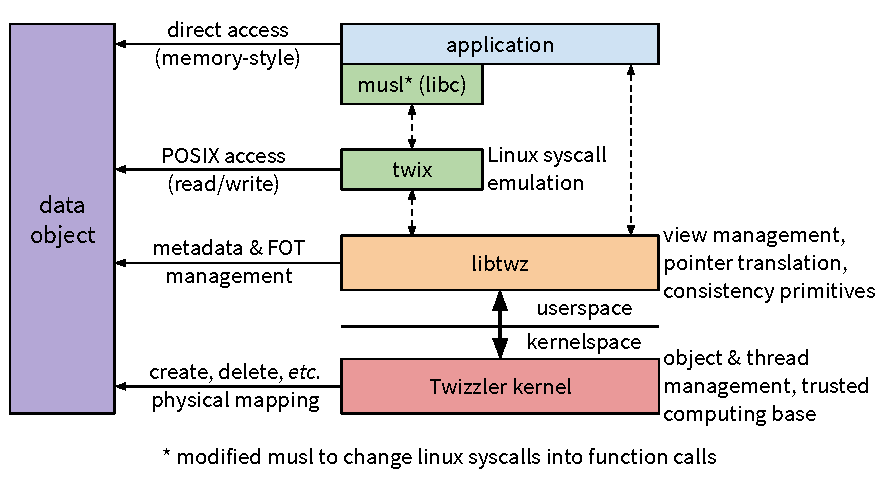
\includegraphics[width=4in]{fig/sys_diag}
        \caption{\Twizzler system overview. Applications link to \texttt{musl} (a C library),
            \texttt{twix} (our Linux syscall emulation library), and \texttt{libtwz} (our standard
            library). Through \texttt{musl}, they may act on persistent data with POSIX interfaces,
            though we expect \Twizzler applications to operate directly on persistent data with
            memory-style semantics.}
        %They can directly access objects or they can use legacy POSIX methods.}
        %The \texttt{libtwz} library provides library-OS functionality and manages the
        %address space and kernel interaction. The kernel manages objects, schedules threads, and
        %enforces security by programming MMU hardware.}
        \label{fig:twz_sys_overview}
    \end{figure}


    \Twizzler's kernel acts much like an
    Exokernel~\cite{Kaashoek,engler:sosp95}, providing sufficient services for a
    userspace library OS, called \emph{\libcore}, to provide an execution environment for applications.
    The primary job of \libcore is to manage mappings of persistent objects into the address space (\S~\ref{sec:view})
    and deal with persistent pointers (\S~\ref{sec:invariant_pointers}).
    \Twizzler also exposes a standard library that
    provides higher level interfaces beyond raw access to memory. For example, software that better fits
    message-passing semantics can use library routines that implement message-passing atop shared
    memory. \Twizzler's standard library provides additional
    higher level interfaces, including streams, logging, event notification, and many
    others. Applications use these to easily build composable tools and pipelines for
    operating on in-memory data structures without the performance loss and complexity of explicit I/O\@.

}

\section{A Historical Look}


\unedit{\label{sec:relwork}

    %The introduction of byte-addressable non-volatile memory presents an outstanding
    %opportunity to rethink the way that OS's handle memory and storage.

    % Working with new technologies often allows past, merely theoretical ideas a
    % chance to be practical.

    \Twizzler's design
    is shaped by fundamental OS
    research~\cite{corbato_introduction_1965,chase:tocs94,k42,engler:sosp95,Kaashoek,engler1995avm,engler1995exterminate},
    which,
    while approaching similar topics described in
    Section~\ref{sec:datacentric}, often did not consider \emph{both} design
    requirements simultaneously, resulting in an incomplete picture for \NVM.
    Recent research on building \NVM data structures~\cite{volos:asplos11,coburn:asplos11,condit:sosp09,debnath:vldb10,lu:tos16,hu:atc17},
    often focuses on building data structures that
    provide failure atomicity and consistency.
    In contrast, we explore how \NVM affects programming models while potentially improving performance.
    We draw from recent work on providing OS support for \NVM systems~\cite{caulfield:micro10} and work
    providing recommendations for \NVM systems~\cite{mehra:ipdps04}, integrating
    object-oriented techniques and simplified kernel design
    to provide high-performance OS support for applications running on a single-level
    store~\cite{shapiro:sosp99,bailey:hotos11}.

    % Our approach will leverage non-volatile memory characteristics to greatly
    % reduce the need for an OS stack and provide full system
    % resumability.
    %, we draw on prior object-oriented OS design work to
    %simplify the kernel using techniques developed in systems such as K42~\cite{k42}
    %and
    %Exokernel~\cite{kaashoek_application_1997, engler:sosp95}.

    %\subsection{Memory Model}
    \paragraph{Memory and Object Model}

    Multics was one of the first systems to use segments to partition memory and
    support relocation~\cite{bensoussan:sosp69,daley:cacm68}. It used segments to
    support location independence, but still stored them in a file system, requiring manual linkage
    rather than the automated linkage in \Twizzler. Nonetheless, Multics demonstrated that the use of
    segmenting for memory management can be a viable approach, though its
    symbolic addresses were slow.

    The core of \Twizzler's object space design uses concepts
    from Opal~\cite{chase:tocs94}, which used a single virtual
    address space for all processes on a system, making it easier to share
    data between programs. However, Opal was a single-address space OS, which is insufficient for
    \NVM~\cite{bittman:plos19,bittman:hotstorage19},
    and, while it resulted in a speedup of data transfer and sharing as well as interfacing with
    devices, it did not address issues of file storage and name resolution. It also
    still required a file
    system, since there was no way to have a pointer refer to an object with changing identity,
    whereas our approach
    of late-binding for pointers
    removes the need for an explicit file system.  Other single-address space
    OSes, such as Mungi~\cite{heiser:scse9314},
    Nemesis~\cite{roscoe:osr94}, and Sombrero~\cite{skousen:ipccc99}, show that
    single address spaces have merit, but, like Opal, did not consider how the use
    of \NVM would alter their design choices; in particular, how the use of fixed addresses
    results in a great deal of coordination that is unnecessary in our approach.
    OSes such as HYDRA~\cite{wulf:cacm74} provide functionality similar to cross-object pointers;
    however, in \Twizzler, we extend their use from procedures-referencing-data to
    a more general approach. Furthermore, they required
    heavy kernel involvement, an approach incompatible with
    our design goals.

    Single-level stores~\cite{shapiro:usenix02,shekita:uwtr956,dearle:cs94} remove the
    memory versus persistent storage distinction, using a single model for data
    at all levels. While well-known,
    ``little has appeared about them in the public
    literature''~\cite{shapiro:usenix02}, even since the EROS paper.
    Our work is partially inspired by Grasshopper~\cite{dearle:cs94}, AS/400, and orthogonal persistence systems,
    but while these are designed to provide an illusion of persistent
    memory, \Twizzler is built for real \NVM and focuses on providing a truly global object space with
    global references without cross-machine coordination.
    Clouds~\cite{dasgupta:computer91} implemented a distributed object store in
    which objects contained code, persistent data, and both volatile and
    persistent heaps. Our approach uses lighter-weight objects, allowing direct
    access to objects from outside, unlike Clouds. Software persistent
    memory~\cite{guerra:atc12}, designed to operate within the constraints
    of existing systems, built a persistent pointer system using explicit
    serialization without cross-object references, in contrast to \Twizzler.
    %In contrast,
    %\Twizzler develops mechanisms that leverage \NVM,
    Meza~\cite{meza:weed13}
    suggested hardware manage a hybrid persistent-volatile store with
    fine-grained movement to and from persistent storage. Since
    persistence in \Twizzler is to \NVM, we need not interpose on
    movement between storage and memory,
    instead simply managing memory mappings of persistent objects,
    reducing OS overhead.

    Recently, several projects have considered the impact of non-volatile
    memories on OS structure. Bailey,
    \etal~\cite{bailey:hotos11} suggest a single-level store design.
    Faraboschi, \etal~\cite{faraboschi:hotos15} discuss challenges and inevitable system organization
    arising from large \NVM, and we follow many of their recommendations.
    %and using
    %\NVM to ship a program as a checkpoint of a running process. 
    The Moneta
    project~\cite{caulfield:micro10} noted that removing the
    heavyweight OS stack dramatically improved performance.
    While Moneta focused on I/O performance, not on rethinking the
    system stack, we leverage their approach to reduce OS
    overhead as much as possible, even when the OS must intervene.
    Lee and Won~\cite{lee:hpcc13} considered the impact of \NVM on
    system initialization by addressing the issue of system boot as a way to restore
    the system to a known state; we may need to include similar techniques to
    address the problem of system corruption.
    Our work evolved from some earlier work where we laid the groundwork for abstraction requirements
    for both hardware and software for \NVM~\cite{bittman:hotstorage19} and a discussion on the
    implications of system-wide persistent data references~\cite{bittman:plos19}.

    \paragraph{Object Model}
    IBM's K42~\cite{k42}
    inspired the high level design of \Twizzler. The
    object-oriented approach to designing a micro or exokernel used in K42 is an
    efficient design for implementing modular OS components.
    Like K42, \Twizzler lazily maps in only the resources that an
    application \emph{needs} to execute. Similar techniques for faulting-in objects at
    run-time have been studied~\cite{Hosking1993}. Communication between objects in
    \Twizzler is, in part, implemented as protected calls, similar to K42.

    Emerald~\cite{jul_implementation_1991,jul:tocs88} and Mesos~\cite{Hindman}
    implemented networked object mobility, which
    we can also support. Emerald implemented a kernel, language, and
    compiler to allow objects mobility using
    wrapper data structures to track metadata and presenting
    objects in an object-oriented language, impacting performance via added indirection for even simple
    operations.

    The \Twizzler object model was shaped by
    NV-heaps~\cite{coburn:asplos11}, which provides memory-safe persistent objects
    suitable for \NVM and describes safety pitfalls in
    providing direct access to \NVM. While they
    have language primitives to enable persistent
    structures, \Twizzler provides a lower-level and uninhibited view of
    objects like Mnemosyne~\cite{volos:asplos11}, allowing
    more powerful programs to be built. Languages and libraries may impose
    further restrictions on \NVM use, but \Twizzler itself does not.
    Furthermore, \Twizzler's cross-object pointers allow external data
    references by code, whereas NV-heap's and DSPM's~\cite{shan:socc17} pointers are
    only internal. Existing work beyond Multics on external references shows and
    recommends hardware support~\cite{wang:micro17,libpmem}, but provides a
    static or per-process view of objects, unlike \Twizzler, limiting scalability and flexibility.
    %and is not used in the context of OS software or
    %libraries.

    Projects such as PMFS~\cite{dulloor:eurosys14} and
    NOVA~\cite{Xu:nova} provide a file system for \NVM. \Twizzler, in
    contrast, provides direct \NVM access atop of a key-value interface of objects.
    Although \Twizzler does not supply a file system, one can be built
    atop it. While NOVA
    and PMFS provide direct access to \NVM, NOVA adds indirection
    with copies. Both use \texttt{mmap} (which falls short as
    discussed above) and, unlike \Twizzler, require significant kernel interaction
    when using persistent memory.

    Our kernel that ``gets out of the way'' is influenced by systems
    such as Exokernel~\cite{engler:sosp95} and SPIN~\cite{bershad:sosp95}, both of
    which drew on Mach~\cite{accetta:usenix86s}. In
    Exokernel, much of the OS is implemented in userspace, with the kernel providing only resource protection. Our approach is
    similar in some respects, but goes further in providing a single unified
    namespace for all objects, making it simpler to develop programs
    that can leverage \NVM to make their state persistent.
    In contrast, SPIN used type-safe languages to provide protection and
    extensibility; our approach cannot rely upon language-provided type safety since
    we want to provide a general purpose platform.

}


\subsection{Single Level Stores}

\subsection{Single Address Space OSes}

\subsection{Distributed Memory and Addressing}